\documentclass{article}

\usepackage{PRIMEarxiv}
\usepackage[utf8]{inputenc}
\usepackage[T1]{fontenc}
\usepackage{hyperref}
\usepackage{url}
\usepackage{booktabs}
\usepackage{amsfonts}
\usepackage{nicefrac}
\usepackage{microtype}
\usepackage{fancyhdr}
\usepackage{graphicx}
\usepackage{amsmath}
\usepackage[table]{xcolor}
\usepackage{float}
\usepackage{placeins}
\usepackage{tikz}
\usepackage{pgfplots}

\usetikzlibrary{arrows.meta,calc,positioning,shapes.geometric}
\pgfplotsset{compat=1.18}

\graphicspath{{figures/}}
\urlstyle{same}

\definecolor{paceNavy}{HTML}{173B63}
\definecolor{paceInk}{HTML}{223044}
\definecolor{paceGold}{HTML}{E9C46A}
\definecolor{paceTeal}{HTML}{2A9D8F}
\definecolor{paceOrange}{HTML}{F4A261}
\definecolor{paceRed}{HTML}{D1495B}
\definecolor{paceGreen}{HTML}{729E4D}
\definecolor{paceBlueLight}{HTML}{DCE7F5}
\definecolor{paceTealLight}{HTML}{D8EEE8}
\definecolor{paceOrangeLight}{HTML}{F6DDD0}
\definecolor{paceGreenLight}{HTML}{DCEAD5}
\definecolor{paceGray}{HTML}{D5DADF}
\setlength{\emergencystretch}{2em}

\newcommand{\tighttable}[1]{%
  \begingroup
  \setlength{\tabcolsep}{5pt}%
  \renewcommand{\arraystretch}{1.12}%
  #1%
  \endgroup
}

\pagestyle{fancy}
\thispagestyle{empty}
\rhead{\textit{Pangu-ACE: Adaptive Cascaded Experts on EduBench}}

\title{Pangu-ACE: Adaptive Cascaded Experts for Educational Response Generation on EduBench}

\author{
  Pangu-ACE Project Team
}

\begin{document}
\maketitle

\begin{abstract}
Educational assistants should spend more computation only when the task needs it. This paper rewrites our earlier draft around the system that was actually implemented and archived in the repository: a sample-level \texttt{1B} $\rightarrow$ \texttt{7B} cascade for the shared-8 EduBench benchmark. The final system, \textbf{Pangu-ACE}, uses a \texttt{1B} tutor-router to produce a draft answer plus routing signals, then either accepts the draft or escalates the sample to a \texttt{7B} specialist prompt. We also correct a major offline evaluation bug: earlier summaries over-credited some open-form outputs that only satisfied superficial format checks. After CPU-side rescoring from saved prediction JSONL, the full Chinese test archive (\(7013\) samples) shows that \texttt{cascade\_final} improves deterministic quality from \(0.457\) to \(0.538\) and format validity from \(0.707\) to \(0.866\) over the legacy \texttt{rule\_v2} system while accepting \(19.7\%\) of requests directly at \texttt{1B}. Routing is strongly task dependent: \texttt{IP} is accepted by \texttt{1B} \(78.0\%\) of the time, while \texttt{QG} and \texttt{EC} still escalate almost always. The current archived deployment does not yet show latency gains, so the defensible efficiency story is routing selectivity rather than wall-clock speedup. We also package a reproducible artifact-first paper workflow and clarify the remaining external-baseline gap: GPT-5.4 re-judging is implemented locally, but the configured provider endpoint and key are invalid, so final sampled-baseline alignment with GPT-5.4 remains pending infrastructure repair.
\end{abstract}

\keywords{Educational agents \and LLM routing \and cascade systems \and EduBench \and offline evaluation}

\section{Introduction}
Educational tasks are structurally heterogeneous. A short factual question, a grading rubric, a personalized study plan, and a teaching-material outline should not all consume the same inference budget, nor should they be judged with the same output contract. That heterogeneity makes education a natural setting for sample-level routing: the system should spend more computation only when the task demands it.

The repository underlying this paper is not a generic agent demo. It is a paper-first offline benchmark stack with deterministic shared-8 EduBench splits, traceable per-sample predictions, and CPU-side recomputation from saved artifacts. The implemented system centers on a calibrated \texttt{1B} $\rightarrow$ \texttt{7B} cascade rather than the quantization-heavy design described in an earlier draft. A lightweight \texttt{1B} stage produces a draft answer together with routing signals; a \texttt{7B} specialist prompt is invoked only for higher-risk samples. This design is closer in spirit to cost-aware routing methods such as FrugalGPT and RouteLLM \cite{frugalgpt, routellm}, but adapted to educational task families and structured output contracts.

Rewriting the paper around the actual code and artifacts reveals a second issue: the original offline summaries overstated quality on open-form tasks. The bug was simple but consequential. Outputs that looked syntactically valid, including router scaffolding such as literal \texttt{draft\_answer} placeholders, were sometimes counted as successful final responses. We therefore rebuilt the paper around rescored predictions, stricter parsing, and explicit limitations.

This revision makes four contributions:
\begin{enumerate}
    \item We present \textbf{Pangu-ACE}, the implemented adaptive cascade used in the final EduBench experiments, with explicit task-family routing and specialist refinement.
    \item We define the paper's benchmark protocol around the shared-8 EduBench tasks and deterministic saved-artifact analysis rather than ad hoc online evaluation.
    \item We correct the offline metric bug for open-form tasks and recompute the paper's quantitative results from raw prediction files.
    \item We diagnose the missing GPT-5.4 baseline path as a provider-configuration failure, not a scoring-pipeline failure, and provide a reproducible re-judge workflow once valid credentials exist.
\end{enumerate}

\section{Benchmark and System}
\subsection{Shared-8 EduBench Setup}
We use the shared-8 EduBench task set \cite{edubench}: \texttt{Q\&A}, \texttt{AG}, \texttt{EC}, \texttt{IP}, \texttt{PCC}, \texttt{PLS}, \texttt{QG}, and \texttt{TMG}. The benchmark excludes \texttt{ES} from the main paper because it is not present symmetrically across the archived Chinese and English assets. The deterministic split plan in the repository fixes the Chinese shared-8 total at \(7793\) samples and the English shared-8 total at \(8102\), with seed \(42\) stratification and frozen dev/test assignments.

The main archived result used in this paper is the full Chinese test split of \(7013\) samples. Only \texttt{cascade\_final} and \texttt{rule\_v2} were fully preserved for that split, so the main table isolates whether the new routing stack improves over the legacy system on exactly the same artifact pool. To retain context for \texttt{1B}-only and \texttt{7B}-only behavior, we also use the preserved fast diagnostic subsets: \(354\) Chinese test samples and \(368\) English test samples.

\subsection{Pangu-ACE Pipeline}
Figure \ref{fig:system_overview} shows the final pipeline. The core design is sample-level semantic routing, not token-level speculative decoding:
\begin{enumerate}
    \item \textbf{Request normalization}: map each EduBench sample to a shared schema with task key, task family, language, expected output format, and prompt text.
    \item \textbf{1B tutor-router}: generate a low-cost draft answer plus routing metadata such as task-family prediction, confidence, and format signals.
    \item \textbf{Risk calibration}: compare the sample's risk score against frozen thresholds obtained on the dev split.
    \item \textbf{Specialist refinement}: if the sample is high risk, pass the original request together with the \texttt{1B} draft to a \texttt{7B} specialist prompt organized by task family (reasoning, assessment, planning).
    \item \textbf{Validation and repair}: normalize the final output, reject router scaffolds and placeholders, and save all artifacts for later CPU-side analysis.
\end{enumerate}

\begin{figure}[H]
  \centering
  \resizebox{0.98\linewidth}{!}{%
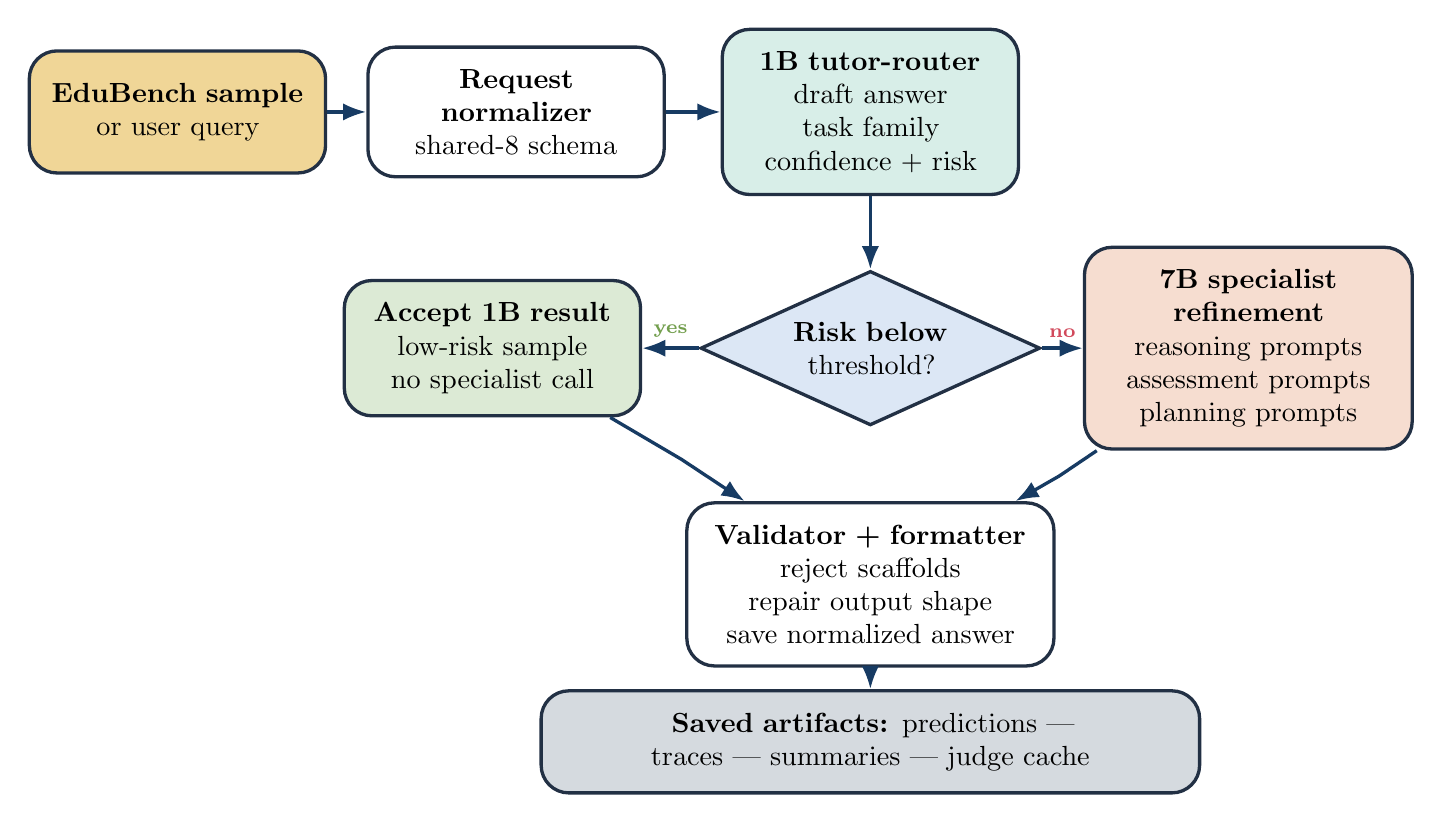
\begin{tikzpicture}[
  x=1cm,
  y=1cm,
  >=Latex,
  line/.style={-Latex, very thick, draw=paceNavy},
  box/.style={
    rounded corners=10pt,
    draw=paceInk,
    very thick,
    align=center,
    minimum height=1.55cm,
    text width=3.2cm,
    inner sep=8pt,
    fill=white
  },
  goldbox/.style={box, fill=paceGold!70},
  tealbox/.style={box, fill=paceTealLight},
  greenbox/.style={box, fill=paceGreenLight},
  orangebox/.style={box, fill=paceOrangeLight, text width=3.6cm},
  whitewide/.style={box, text width=4.1cm},
  graybox/.style={box, fill=paceGray, text width=7.8cm, minimum height=1.0cm},
  decision/.style={
    diamond,
    aspect=2.2,
    draw=paceInk,
    very thick,
    fill=paceBlueLight,
    align=center,
    inner sep=2pt,
    text width=2.4cm
  }
]
\node[goldbox]   (query)      at (0.0,  0.0)  {\textbf{EduBench sample}\\or user query};
\node[box]       (norm)       at (4.3,  0.0)  {\textbf{Request normalizer}\\shared-8 schema};
\node[tealbox]   (router)     at (8.8,  0.0)  {\textbf{1B tutor-router}\\draft answer\\task family\\confidence + risk};
\node[decision]  (decision)   at (8.8, -3.0)  {\textbf{Risk below}\\threshold?};
\node[greenbox]  (accept)     at (4.0, -3.0)  {\textbf{Accept 1B result}\\low-risk sample\\no specialist call};
\node[orangebox] (specialist) at (13.6,-3.0)  {\textbf{7B specialist refinement}\\reasoning prompts\\assessment prompts\\planning prompts};
\node[whitewide] (validator)  at (8.8, -6.0)  {\textbf{Validator + formatter}\\reject scaffolds\\repair output shape\\save normalized answer};
\node[graybox]   (artifacts)  at (8.8, -8.0)  {\textbf{Saved artifacts:} predictions | traces | summaries | judge cache};

\draw[line] (query) -- (norm);
\draw[line] (norm) -- (router);
\draw[line] (router) -- (decision);
\draw[line] (decision) -- node[midway, above, font=\scriptsize\bfseries, text=paceGreen] {yes} (accept);
\draw[line] (decision) -- node[midway, above, font=\scriptsize\bfseries, text=paceRed] {no} (specialist);
\draw[line] (accept) -- ($(accept.south)!0.5!(validator.north)$) -- (validator);
\draw[line] (specialist) -- ($(specialist.south)!0.5!(validator.north)$) -- (validator);
\draw[line] (validator) -- (artifacts);
\end{tikzpicture}%
}

  \caption{Implemented Pangu-ACE pipeline. A normalized EduBench sample is drafted by the \texttt{1B} tutor-router, scored by the calibrator, then either accepted directly or sent to a \texttt{7B} specialist before final validation and artifact logging.}
  \label{fig:system_overview}
\end{figure}
\FloatBarrier

The system's strength is not universal. It is best viewed as a calibrated routing layer on top of specialist prompting. Strong planning and generation tasks still depend heavily on \texttt{7B}, while idea prompting and parts of personalized learning are often handled successfully by \texttt{1B}.

\section{Evaluation Protocol and Metric Correction}
\subsection{Artifact-First Evaluation}
The paper follows the repository's artifact-first protocol: run inference once, save prediction JSONL and trace JSONL, then regenerate summaries later without re-running GPUs. This matters because the current paper is built after the experimental runs were finished. The rewritten tables and figures are produced from saved artifacts in \path{outputs/predictions/} and \path{outputs/traces/}, not from manually copied console logs.

\subsection{Corrected Deterministic Quality}
Closed-form tasks and open-form tasks need different deterministic checks. For \texttt{Q\&A}, \texttt{AG}, and \texttt{EC}, we use exact or field-level comparison against the ground truth. For open-form tasks, we use a stricter criterion than the earlier draft:
\[
q_i =
\begin{cases}
1[\hat{y}_i = y_i], & \text{for } \texttt{Q\&A}, \texttt{AG}, \texttt{EC} \\
1[\mathrm{valid}(\hat{y}_i) \land \mathrm{substantive}(\hat{y}_i)], & \text{for } \texttt{IP}, \texttt{PCC}, \texttt{PLS}, \texttt{QG}, \texttt{TMG}
\end{cases}
\]
where \(\mathrm{substantive}(\hat{y}_i)\) rejects placeholders, router scaffolding, and malformed nested drafts. This correction matters because superficially valid JSON should not count as a successful educational response when its content is only a scaffold.

We report four families of metrics:
\begin{itemize}
    \item \textbf{Quality}: the deterministic score above, averaged over the relevant samples.
    \item \textbf{Format validity}: whether the output satisfies the expected schema after normalization.
    \item \textbf{Routing rates}: \texttt{1B} acceptance and \texttt{7B} invocation extracted from saved traces.
    \item \textbf{Latency}: archived end-to-end latency per sample. This reflects the detached service setup that was actually used during the runs.
\end{itemize}

\section{Results}
\subsection{Main Archived Chinese Test}
Table \ref{tab:main_zh} is the paper's primary quantitative result. On the same \(7013\)-sample Chinese test archive, \texttt{cascade\_final} raises quality by \(+0.081\) absolute and format validity by \(+0.159\) absolute over \texttt{rule\_v2}. It also accepts \(19.7\%\) of requests directly at \texttt{1B}, reducing the fraction that reaches the \texttt{7B} stage from \(100\%\) to \(80.3\%\).

The trade-off is equally important: end-to-end latency is \emph{higher} for the cascade in the current deployment (\(26.35\)s vs. \(18.33\)s). The paper therefore should not claim a latency win. The defensible claim is narrower and more useful: the new system buys better quality and cleaner outputs while demonstrating selective \texttt{7B} usage. Recovering wall-clock gains will require implementation work beyond routing itself, such as fusing the router stage, reducing orchestration overhead, or shortening specialist outputs.

\begin{table}[H]
\centering
\caption{Full Chinese test results after rescoring saved predictions.}
\label{tab:main_zh}
\small
\tighttable{\begin{tabular}{lrrrrrr}
\toprule
System & Samples & Quality & Format & Latency (s) & 7B rate & 1B accept \\
\midrule
\texttt{rule\_v2} & 7013 & 0.457 & 0.707 & 18.33 & 100.0\% & -- \\
\rowcolor{paceTealLight}
\texttt{cascade\_final} & 7013 & \textbf{0.538} & \textbf{0.866} & 26.35 & \textbf{80.3\%} & \textbf{19.7\%} \\
\bottomrule
\end{tabular}
}
\end{table}
\FloatBarrier

\subsection{Fast Diagnostic Baselines}
The fast diagnostic subsets provide the missing baselines that were not archived on the full Chinese test. On the Chinese subset, \texttt{7b\_only} reaches quality \(0.591\) and \texttt{cascade\_final} reaches \(0.510\) while invoking \texttt{7B} on \(77.1\%\) of samples. On the English subset, \texttt{7b\_only} reaches \(0.534\) and \texttt{cascade\_final} reaches \(0.472\) with \texttt{7B} invocation at \(85.3\%\). \texttt{1b\_only} is consistently much weaker in both languages.

Figure \ref{fig:quality_latency} summarizes the resulting quality-latency frontier. The current archived cascade is not faster than \texttt{7b\_only}; in fact it is slower because the extra routing stage adds orchestration cost. The value of the figure is therefore diagnostic rather than celebratory: it shows that the routing stack is not yet a free lunch. We gain selectivity, but we have not yet converted that selectivity into latency savings.

\begin{figure}[H]
  \centering
  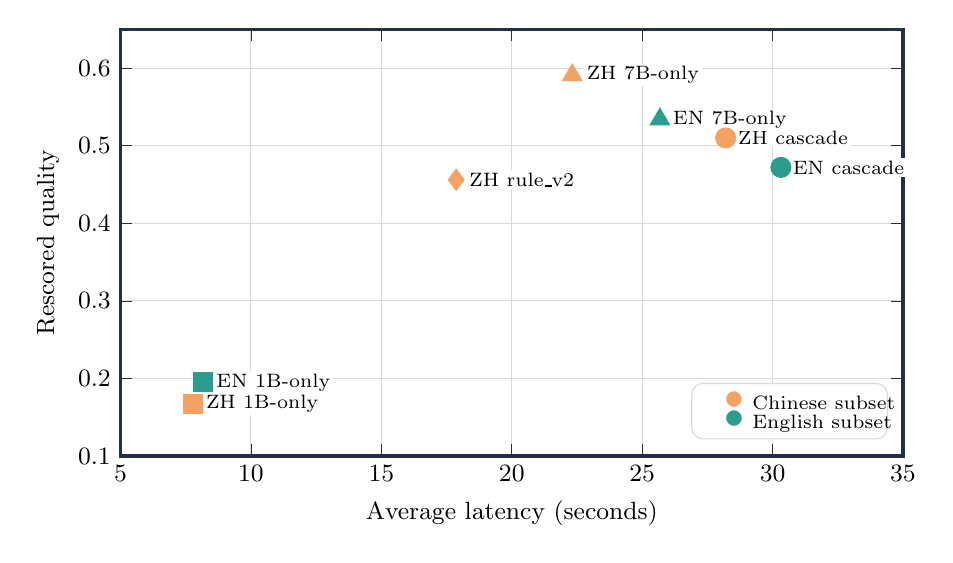
\begin{tikzpicture}
\begin{axis}[
  width=0.95\linewidth,
  height=7.0cm,
  xmin=5,
  xmax=35,
  ymin=0.10,
  ymax=0.65,
  xlabel={Average latency (seconds)},
  ylabel={Rescored quality},
  axis line style={draw=paceInk, very thick},
  tick style={draw=paceInk},
  tick label style={font=\small},
  label style={font=\small},
  grid=major,
  major grid style={draw=paceGray},
  clip=false
]
\addplot[only marks, mark=square*, mark size=3.4pt, color=paceOrange] coordinates {(7.77,0.167)};
\node[anchor=west, font=\scriptsize, fill=white, inner sep=1pt] at (axis cs:8.15,0.167) {ZH 1B-only};

\addplot[only marks, mark=diamond*, mark size=3.8pt, color=paceOrange] coordinates {(17.87,0.456)};
\node[anchor=west, font=\scriptsize, fill=white, inner sep=1pt] at (axis cs:18.25,0.456) {ZH rule\_v2};

\addplot[only marks, mark=*, mark size=3.6pt, color=paceOrange] coordinates {(28.20,0.510)};
\node[anchor=west, font=\scriptsize, fill=white, inner sep=1pt] at (axis cs:28.55,0.510) {ZH cascade};

\addplot[only marks, mark=triangle*, mark size=4.0pt, color=paceOrange] coordinates {(22.32,0.591)};
\node[anchor=west, font=\scriptsize, fill=white, inner sep=1pt] at (axis cs:22.75,0.591) {ZH 7B-only};

\addplot[only marks, mark=square*, mark size=3.4pt, color=paceTeal] coordinates {(8.15,0.195)};
\node[anchor=west, font=\scriptsize, fill=white, inner sep=1pt] at (axis cs:8.55,0.195) {EN 1B-only};

\addplot[only marks, mark=*, mark size=3.6pt, color=paceTeal] coordinates {(30.32,0.472)};
\node[anchor=west, font=\scriptsize, fill=white, inner sep=1pt] at (axis cs:30.65,0.472) {EN cascade};

\addplot[only marks, mark=triangle*, mark size=4.0pt, color=paceTeal] coordinates {(25.68,0.534)};
\node[anchor=west, font=\scriptsize, fill=white, inner sep=1pt] at (axis cs:26.05,0.534) {EN 7B-only};

\draw[draw=paceGray, rounded corners=4pt, fill=white] (rel axis cs:0.73,0.04) rectangle (rel axis cs:0.98,0.17);
\node[anchor=west, font=\scriptsize] at (rel axis cs:0.76,0.13) {\textcolor{paceOrange}{\Large$\bullet$} Chinese subset};
\node[anchor=west, font=\scriptsize] at (rel axis cs:0.76,0.08) {\textcolor{paceTeal}{\Large$\bullet$} English subset};
\end{axis}
\end{tikzpicture}

  \caption{Quality-latency trade-off on the preserved fast diagnostic subsets. The present cascade improves strongly over \texttt{1b\_only}, but it still trails \texttt{7b\_only} in wall-clock latency because routing overhead is not yet amortized.}
  \label{fig:quality_latency}
\end{figure}
\FloatBarrier

\subsection{Routing Behavior by Task}
The routing analysis in Figure \ref{fig:routing_by_task} explains why the cascade is still worthwhile. The system is not uniformly conservative. It accepts \texttt{IP} samples directly at \texttt{1B} \(78.0\%\) of the time, \texttt{PLS} \(35.5\%\), and \texttt{Q\&A} \(25.9\%\). In contrast, \texttt{EC} and \texttt{QG} escalate every sample, and \texttt{TMG} escalates \(99.6\%\) of them. This is the right qualitative pattern for the current prompt inventory: ideation is relatively draft-friendly, while generation and correction tasks remain specialist-heavy.

\begin{figure}[H]
  \centering
  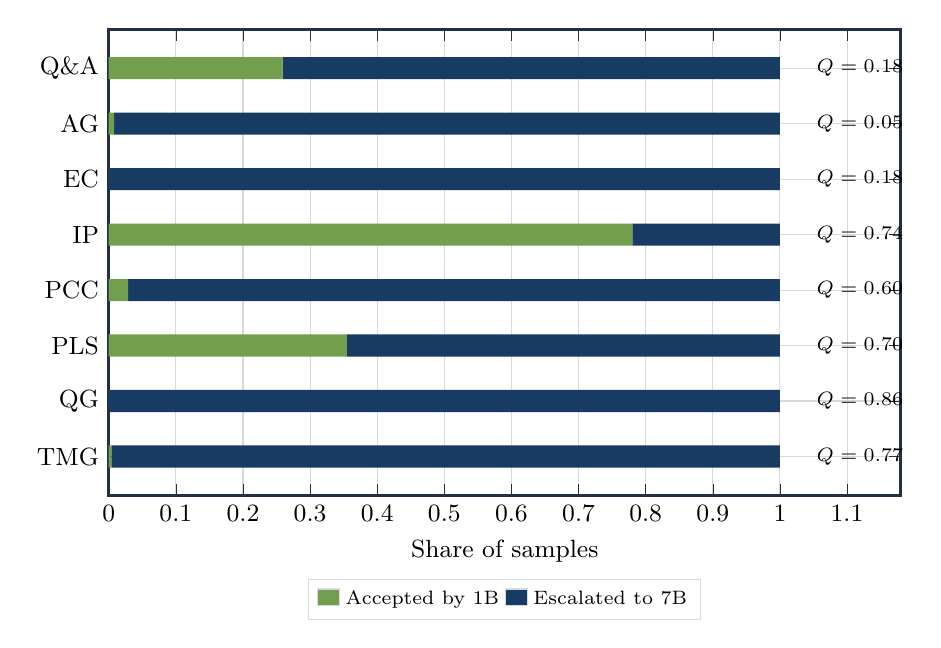
\begin{tikzpicture}
\begin{axis}[
  width=0.96\linewidth,
  height=7.5cm,
  xbar stacked,
  xmin=0,
  xmax=1.18,
  symbolic y coords={Q\&A,AG,EC,IP,PCC,PLS,QG,TMG},
  ytick=data,
  y dir=reverse,
  bar width=8pt,
  xlabel={Share of samples},
  axis line style={draw=paceInk, very thick},
  tick style={draw=paceInk},
  tick label style={font=\small},
  label style={font=\small},
  grid=major,
  major grid style={draw=paceGray},
  legend style={draw=paceGray, fill=white, font=\scriptsize, at={(0.5,-0.18)}, anchor=north, legend columns=2},
  clip=false
]
\addplot[fill=paceGreen, draw=none] coordinates {
  (0.259,Q\&A)
  (0.008,AG)
  (0.000,EC)
  (0.780,IP)
  (0.029,PCC)
  (0.355,PLS)
  (0.000,QG)
  (0.004,TMG)
};
\addplot[fill=paceNavy, draw=none] coordinates {
  (0.741,Q\&A)
  (0.992,AG)
  (1.000,EC)
  (0.220,IP)
  (0.971,PCC)
  (0.645,PLS)
  (1.000,QG)
  (0.996,TMG)
};
\legend{Accepted by 1B,Escalated to 7B}

\node[anchor=west, font=\scriptsize] at (axis cs:1.04,Q\&A) {$Q=0.18$};
\node[anchor=west, font=\scriptsize] at (axis cs:1.04,AG) {$Q=0.05$};
\node[anchor=west, font=\scriptsize] at (axis cs:1.04,EC) {$Q=0.18$};
\node[anchor=west, font=\scriptsize] at (axis cs:1.04,IP) {$Q=0.74$};
\node[anchor=west, font=\scriptsize] at (axis cs:1.04,PCC) {$Q=0.60$};
\node[anchor=west, font=\scriptsize] at (axis cs:1.04,PLS) {$Q=0.70$};
\node[anchor=west, font=\scriptsize] at (axis cs:1.04,QG) {$Q=0.86$};
\node[anchor=west, font=\scriptsize] at (axis cs:1.04,TMG) {$Q=0.77$};
\end{axis}
\end{tikzpicture}

  \caption{Routing mix on the full Chinese test archive. Bars show how often each task is accepted at \texttt{1B} or escalated to \texttt{7B}; the annotation on the right reports rescored quality for the same task.}
  \label{fig:routing_by_task}
\end{figure}
\FloatBarrier

\subsection{Task-Level Gains and Failure Modes}
Figure \ref{fig:task_delta} compares per-task quality against the legacy \texttt{rule\_v2} baseline on the full Chinese archive. The cascade helps most on generation-heavy tasks: \texttt{QG} improves by \(+0.265\) and \texttt{TMG} by \(+0.366\). It is also slightly better on \texttt{EC} and \texttt{IP}. The weak spots are equally informative. \texttt{PLS} drops well below the legacy rule system, and \texttt{AG} remains poor for both systems. These results suggest that the next round of work should focus on grading prompts and personalized-learning templates rather than further broadening the routing stack.

\begin{figure}[H]
  \centering
  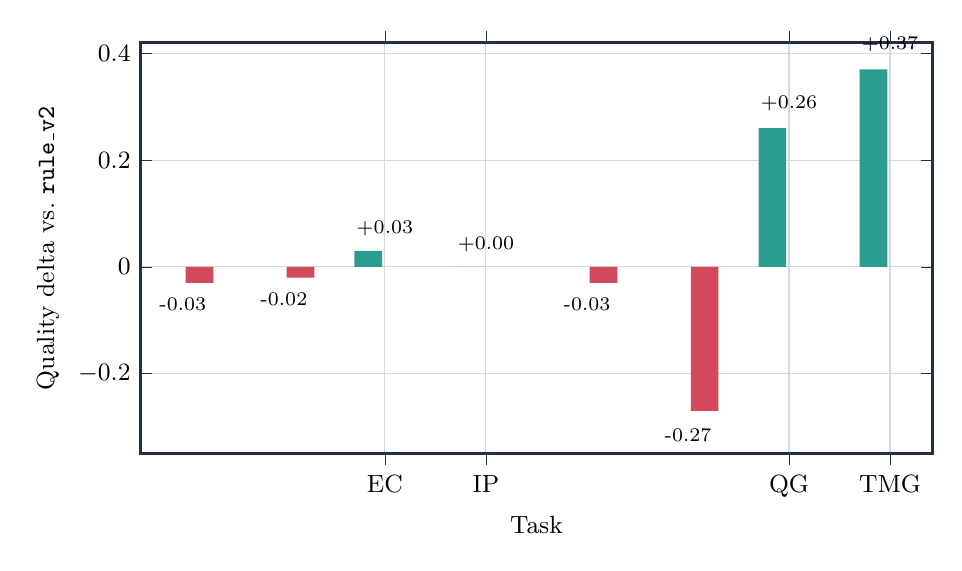
\begin{tikzpicture}
\begin{axis}[
  width=0.96\linewidth,
  height=6.8cm,
  ybar,
  ymin=-0.35,
  ymax=0.42,
  symbolic x coords={Q\&A,AG,EC,IP,PCC,PLS,QG,TMG},
  xtick=data,
  xlabel={Task},
  ylabel={Quality delta vs.\ \texttt{rule\_v2}},
  axis line style={draw=paceInk, very thick},
  tick style={draw=paceInk},
  tick label style={font=\small},
  x tick label style={rotate=0, anchor=north},
  label style={font=\small},
  grid=major,
  major grid style={draw=paceGray},
  enlarge x limits=0.06,
  bar width=10pt,
  clip=false
]
\addplot[fill=paceTeal, draw=none] coordinates {
  (EC,0.03)
  (IP,0.00)
  (QG,0.26)
  (TMG,0.37)
};
\addplot[fill=paceRed, draw=none] coordinates {
  (Q\&A,-0.03)
  (AG,-0.02)
  (PCC,-0.03)
  (PLS,-0.27)
};

\node[font=\scriptsize, anchor=south] at (axis cs:EC,0.04) {+0.03};
\node[font=\scriptsize, anchor=south] at (axis cs:IP,0.01) {+0.00};
\node[font=\scriptsize, anchor=south] at (axis cs:QG,0.275) {+0.26};
\node[font=\scriptsize, anchor=south] at (axis cs:TMG,0.385) {+0.37};

\node[font=\scriptsize, anchor=north] at (axis cs:Q\&A,-0.04) {-0.03};
\node[font=\scriptsize, anchor=north] at (axis cs:AG,-0.03) {-0.02};
\node[font=\scriptsize, anchor=north] at (axis cs:PCC,-0.04) {-0.03};
\node[font=\scriptsize, anchor=north] at (axis cs:PLS,-0.285) {-0.27};
\end{axis}
\end{tikzpicture}

  \caption{Per-task quality delta of \texttt{cascade\_final} relative to \texttt{rule\_v2} on the full Chinese test archive. The largest gains are on question generation and teaching-material generation; grading and personalized learning remain weak points.}
  \label{fig:task_delta}
\end{figure}
\FloatBarrier

\section{External EduBench Baselines and GPT-5.4 Status}
The repository also contains the official EduBench sampled baseline scores in \path{EduBench/data/all_data/model_eval_score/model_sampled_eval_scores.csv}. We aggregated those rows into paper-ready tables to retain external context. Under the existing \texttt{gpt-4o} evaluator, the strongest available sampled baseline is DeepSeek R1 with an average score of \(9.05\), followed by Qwen Max (\(9.00\)) and DeepSeek V3 (\(8.99\)); Table \ref{tab:edubench_reference} lists representative scenario-level scores.

These reference numbers are useful, but they are \emph{not directly comparable} to the deterministic \(0\)-to-\(1\) quality metric used in our current paper tables. They are sampled-response judge scores on a \(1\)-to-\(10\) scale. The correct way to align them is to re-judge the same sampled baseline responses with the desired evaluator and aggregate them into the same CSV shape.

That path is implemented locally, but as of \textbf{March 16, 2026} it remains blocked by provider configuration. The current default \texttt{GPT5\_API\_BASE} points to \url{https://api.aicodemirror.com/v1}, and probe requests to \texttt{/models}, \texttt{/chat/completions}, and \texttt{/responses} return \texttt{404}. The current secret also has an Anthropic-style prefix (\texttt{sk-ant-}), which does not match the OpenAI-compatible interface expected by the re-judge code. The missing GPT-5.4 baseline table is therefore an infrastructure issue, not an evaluation-code issue.

\begin{table}[H]
\centering
\caption{Official EduBench sampled baseline reference under the GPT-4o evaluator. These values come from the provided baseline CSV and are shown as external context only.}
\label{tab:edubench_reference}
\small
\tighttable{\begin{tabular}{lrrrrrr}
\toprule
Model & Avg. & Q\&A & IP & AG & QG & PCC \\
\midrule
\rowcolor{paceTealLight}
DeepSeek R1 & \textbf{9.05} & 9.32 & 8.78 & 8.51 & 8.98 & \textbf{9.08} \\
Qwen Max & 9.00 & \textbf{9.50} & 8.69 & \textbf{8.70} & 8.92 & 9.05 \\
DeepSeek V3 & 8.99 & 9.22 & 8.77 & 8.54 & \textbf{9.00} & 8.95 \\
Qwen2.5-14B-Instruct & 8.87 & 9.34 & 8.51 & 8.11 & 8.77 & 8.82 \\
Qwen2.5-7B-Instruct & 8.86 & 9.22 & \textbf{8.84} & 8.04 & 8.62 & 8.94 \\
\bottomrule
\end{tabular}
}
\end{table}
\FloatBarrier

\section{Limitations and Conclusion}
This paper revision is deliberately narrower than the original draft. It reports what the archived artifacts actually support:
\begin{itemize}
    \item The full main table is Chinese only because that is the only split with full archived \texttt{cascade\_final} and \texttt{rule\_v2} predictions after correction.
    \item The \texttt{1B}-only and \texttt{7B}-only baselines are diagnostic rather than archival full-benchmark runs.
    \item Routing selectivity is real, but it has not yet translated into wall-clock gains in the detached deployment used for the experiments.
    \item External sampled-baseline alignment with GPT-5.4 remains pending a valid provider configuration.
\end{itemize}

Even with these limits, the paper now tells a coherent and defensible story. Pangu-ACE is a real educational cascade, not a placeholder architecture. Its saved artifacts support a clear conclusion: a calibrated \texttt{1B} $\rightarrow$ \texttt{7B} pipeline improves output quality and output validity over the legacy rule system while showing meaningful task-dependent routing behavior. The next engineering milestone is not another model role; it is to make the current routing savings visible in wall-clock performance and to finish the GPT-5.4 baseline alignment once the provider configuration is repaired.

\appendix
\clearpage
\section{Supplementary Tables}
We include the preserved fast diagnostic and ablation tables for completeness. The ablation subset is small (\(178\) Chinese samples), so we treat it as directional evidence rather than a final ranking of components.

\begin{table}[H]
\centering
\caption{Chinese fast diagnostic subset.}
\small
\tighttable{\begin{tabular}{lrrrrrr}
\toprule
System & Samples & Quality & Format & Latency (s) & 7B rate & 1B accept \\
\midrule
\texttt{1b\_only} & 354 & 0.167 & 0.220 & 7.77 & 0.0\% & 100.0\% \\
\texttt{rule\_v2} & 354 & 0.456 & 0.686 & 17.87 & 100.0\% & -- \\
\rowcolor{paceTealLight}
\texttt{cascade\_final} & 354 & 0.510 & 0.833 & 28.20 & \textbf{77.1\%} & \textbf{22.9\%} \\
\texttt{7b\_only} & 354 & \textbf{0.591} & \textbf{0.847} & 22.32 & 100.0\% & -- \\
\bottomrule
\end{tabular}
}
\end{table}

\begin{table}[H]
\centering
\caption{English fast diagnostic subset.}
\small
\tighttable{\begin{tabular}{lrrrrrr}
\toprule
System & Samples & Quality & Format & Latency (s) & 7B rate & 1B accept \\
\midrule
\texttt{1b\_only} & 368 & 0.195 & 0.236 & 8.15 & 0.0\% & 100.0\% \\
\rowcolor{paceTealLight}
\texttt{cascade\_final} & 368 & 0.472 & 0.750 & 30.32 & \textbf{85.3\%} & \textbf{14.7\%} \\
\texttt{7b\_only} & 368 & \textbf{0.534} & \textbf{0.785} & 25.68 & 100.0\% & -- \\
\bottomrule
\end{tabular}
}
\end{table}

\begin{table}[H]
\centering
\caption{Chinese ablation subset (\(178\) samples).}
\small
\tighttable{\begin{tabular}{lrrrrr}
\toprule
Variant & Samples & Quality & Format & Latency (s) & 7B rate \\
\midrule
\rowcolor{paceTealLight}
\texttt{cascade\_final} & 178 & 0.569 & 0.843 & 27.68 & 82.0\% \\
w/o calibrator & 178 & 0.574 & 0.865 & 27.08 & 78.1\% \\
w/o specialist prompt & 178 & 0.602 & \textbf{0.921} & \textbf{23.48} & 78.1\% \\
w/o draft conditioning & 178 & \textbf{0.610} & 0.882 & 26.80 & \textbf{73.6\%} \\
\bottomrule
\end{tabular}
}
\end{table}

\bibliographystyle{plain}
\bibliography{references}

\end{document}
